\documentclass[10pt]{beamer}

%STANDARD PREAMBLE
%https://tex.stackexchange.com/questions/68821/is-it-possible-to-create-a-latex-preamble-header
\usepackage{/Users/mwojno01/Repos/latex_preamble/beamer_preamble}

%
%% ALLOW FOR ITEMIZE ENVIRONMENTS WITH NO PRECEDING
% SPACING, IF DESIRED
% Reference: https://tex.stackexchange.com/questions/86054/how-to-remove-the-whitespace-before-itemize-enumerate
%\usepackage{enumitem}% http://ctan.org/pkg/enumitem 
\usepackage{paralist}


\title{Jensen's Inequality}
\subtitle{Intuition and Proof}

\begin{document}

\maketitle


\begin{frame}{Goals}
\begin{enumerate}
	\item Formally state Jensen's inequality.
	\item Provide intuition on the direction of the inequality.
	\item Show how to prove it by representing an arbitrary \alert{convex} function in terms of \alert{linear} functions.
\end{enumerate}
	
\end{frame}

\begin{frame}


\begin{block}{Theorem (Jensen's Inequality)}
Let $g$ be a convex function from $I$ to $\R$, where $I$ is an open interval of reals.  Let $X$ be random variable on $(\Omega, \F, P)$, with $X(\omega) \in I$ for all $\omega$.  Assume $E[X]$ to be finite. If $\mathcal{H}$ is a sub $\sigma$-field of $\F$, then 
%
\begin{align}
\E[g(X) \cond \mathcal{H}] \geq g(\E[X \cond \mathcal{H}]) \quad a.e. 
\label{eqn:jensens_inequality_for_conditional_expectations}	
\end{align}  

In particular, $\E[g(X)] \geq g(\E[X])$.
\label{thm:jensens_inequality}	
\end{block}

\vfill 
\pause 
\begin{block}{How to recall the direction of the inequality {\small [Durrett, 2010]}}

\vskip 0.1in

\begin{columns}
\begin{column}{0.6\textwidth}
{\small
Take $P(X=x) = \lambda$, $P(X=y) = 1-\lambda$.
\begin{align*}
	\E[g(X)] &= \lambda \, g(x) + (1-\lambda) \, g(y) && \tinytext{LOTUS} \\
	& \geq  g \big(\lambda x  + (1-\lambda) y  \big) && \tinytext{def. convexity}\\
		&= g \big( \E[X] \big). && \tinytext{def. expectation} 
\end{align*}
}
\end{column}
\vrule{}
\begin{column}{0.32\textwidth}
    {\scriptsize For example: $P(X=1) = P(X=3) = .5$ } 
    \begin{center}
     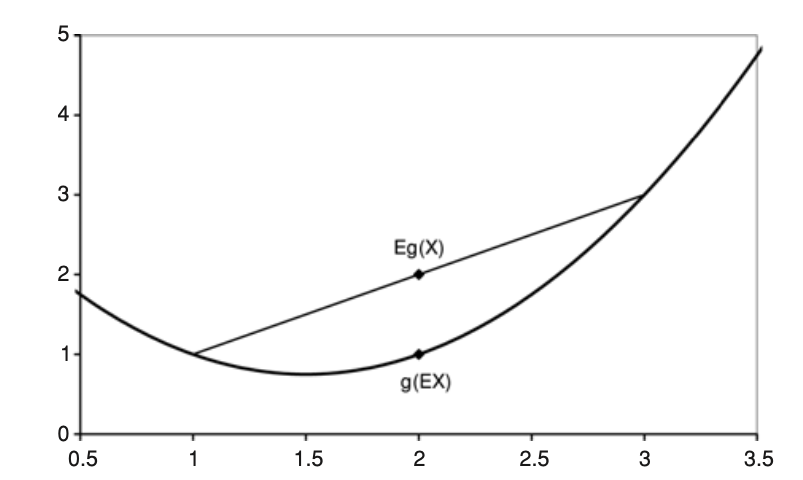
\includegraphics[width=\textwidth]{images/jensens_inequality_per_durrett}  
     \end{center}
\end{column}
%
\end{columns}
\end{block}

\end{frame}

\begin{frame}
\begin{block}{Line of Support Theorem.}  Let $g : I \to \R$, where $I$ is an open interval of reals, bounded or unbounded. Assume $g$ is convex, that is,
\[\explaintermbrace{graph}{g \big(\alpha x + (1-\alpha) y \big)} \leq \explaintermbrace{chord}{\alpha g(x) + (1-\alpha) g(y)} \]
for all $x,y \in I$ and all $\alpha \in [0,1]$.  Then there are sequences $\set{a_n}, \set{b_n}$ of real numbers such that for all $x \in I$, 
\[ g(x) = \sup_n \; (a_n x + b_n)\]
\label{thm:line_of_support}
\end{block}

\begin{figure}[H]
\centering
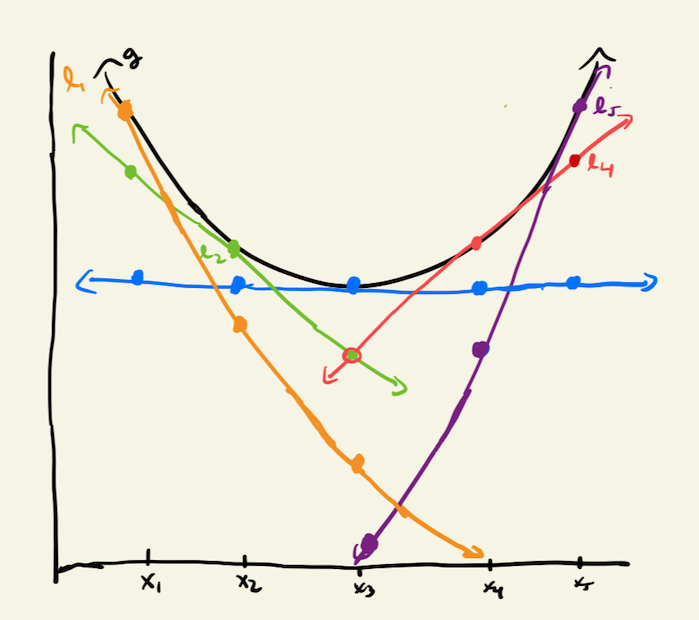
\includegraphics[width=.3\textwidth]{images/line_of_support_theorem}
%\caption{\textit{Cartoon sketch of line of support theorem.}   Shown are a convex function $g$ and five elements of a sequence $\set{\ell_n}$ of lines of support.}
\end{figure}
\end{frame}

\begin{frame}
\begin{block}{Proof (partial)}
Here we show that Jensen's inequality (\Eqref{eqn:jensens_inequality_for_conditional_expectations}) holds.

\begin{align*}
&g(X) = \sup_n \, a_n X + b_n  && \scripttext{Line of Support Theorem (Theorem~\ref{thm:line_of_support})}\\
\implies &g(X) \geq a_n X + b_n && \scripttext{supremum is an upper bound} \\
\implies & \E[g(X) \cond \mathcal{H}] \geq \E[a_n X + b_n \cond \mathcal{H}] \quad  \tinytext{a.e.} &&\scripttext{monotonicity} \\
\implies & \E[g(X) \cond \mathcal{H}] \geq a_n \, \E[X \cond \mathcal{H}] + b_n \quad  \tinytext{a.e.}&&\scripttext{linearity} \\
\implies & \E[g(X) \cond \mathcal{H}] \geq \explaintermbrace{$=g(\E[X \cond \mathcal{H}])$ by LoS Thm.}{\sup_n \set{a_n \, \E[X \cond \mathcal{H}] + b_n}} \quad \tinytext{a.e.}  &&  \scripttext{supremum is least upper bound} 
\end{align*}
\end{block}
\end{frame}

\begin{frame}[standout]
The Line of Support Theorem allows us to take an arbitrary \alert{convex} function and represent it in terms of \alert{linear} functions (and therefore apply properties that hold under linearity). 	
\end{frame}


\end{document}